To evaluate the performance of the robot in terms of completing the engineering challenge a setupr shown in Fig. \ref{fig:factory_setup}. The setup consists of the main factory model and red lines connecting the drop-off point to the left and the pickup point to the right. The read lines specify the path the robot can take. At each endpoint and corner of the colored path a QR-code is placed which contains an coordinate of that point in space. The goal for the robot is to receive an instruction from Arrowhead, either to pickup the piece on the platform or drop it off in the drop off area. The robot would then navigate autonomously to the correct coordinate and perform the pick up or drop off action with the arm. 

\begin{figure}
    \centering
    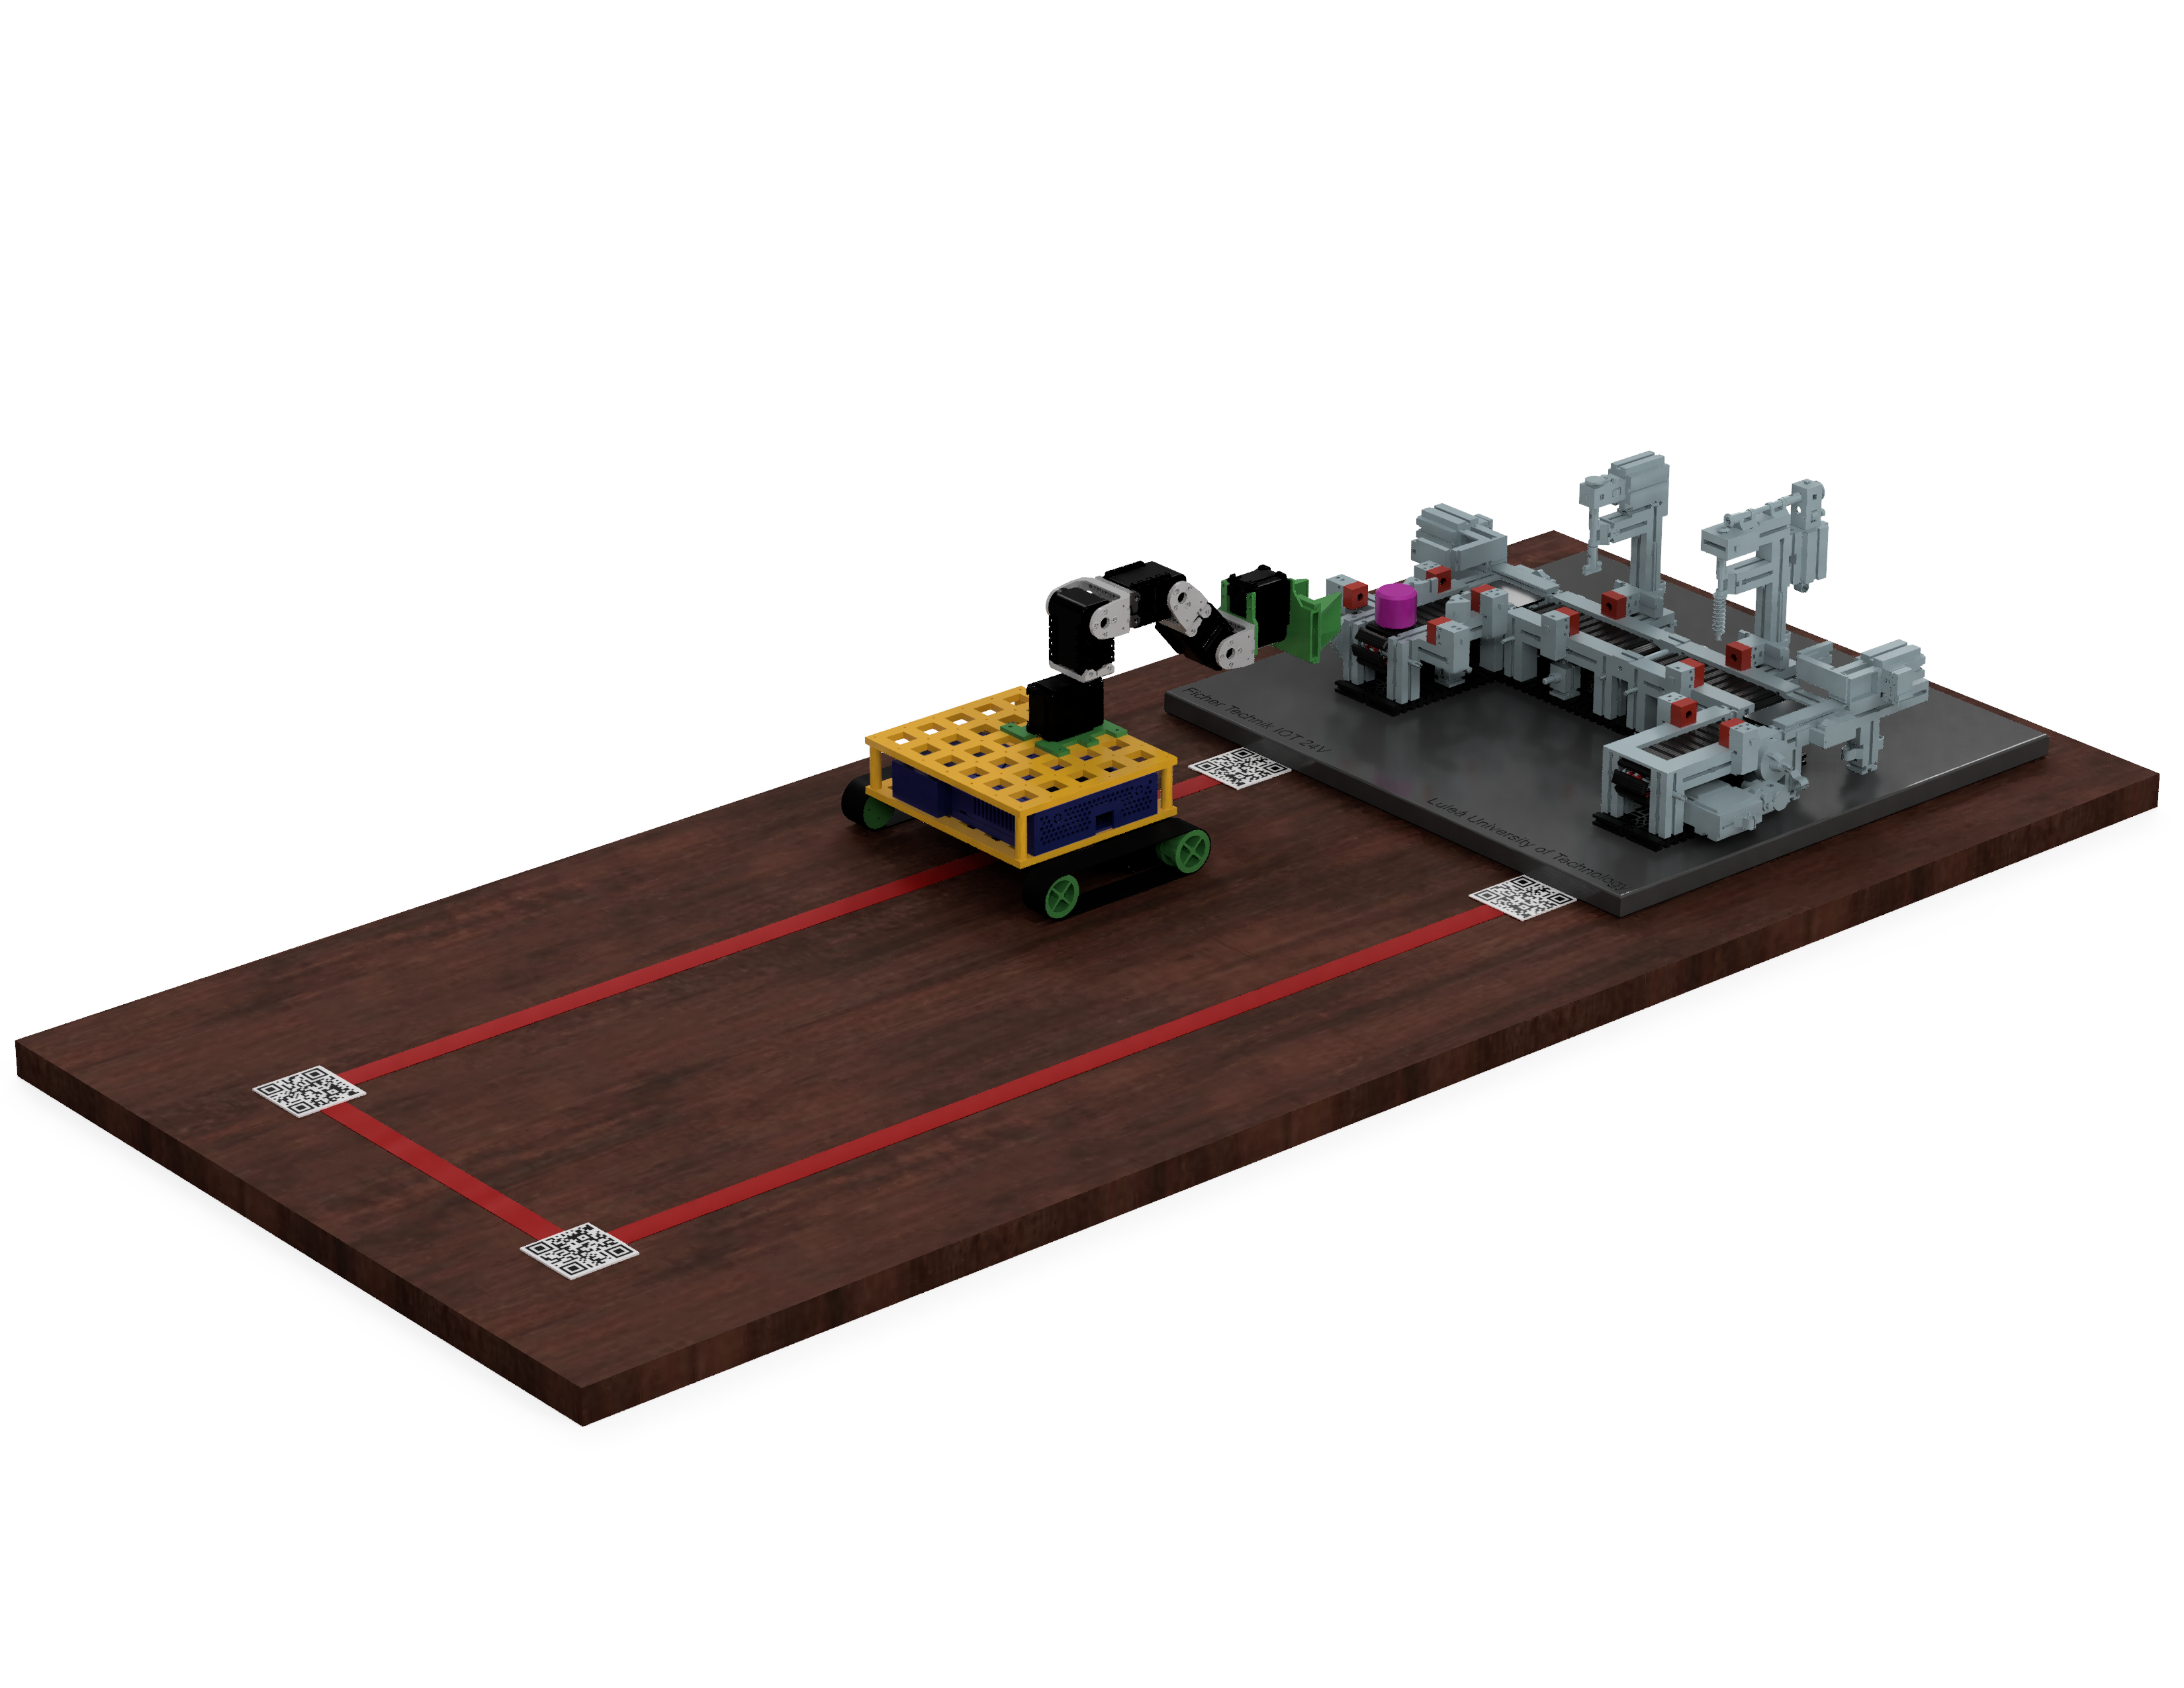
\includegraphics[width=0.7\columnwidth]{chapters/img/evaluation_setup.png}
    \caption{Rendering of concept design.}
    \label{fig:factory_setup}
\end{figure}